\subsection{Overview}
The following chapter presents the findings of a comparative analysis of mobile application development using Java, Kotlin, and Dart (Flutter). The study primarily focuses on the SonarQube code quality assessments of identical Kanban board applications developed in each framework. The severity of code smells and other metrics, such as the model of Task implementation in all three frameworks, were analyzed in detail. Accompanying tables and severity graphs provide a quantified representation of these findings. Additionally, the chapter offers insights into the practical differences between the frameworks, considering the application size and pertinent notes on the development process.
\par
Further, the study delves into the implementation of SonarQube across a selection of open-source projects developed in Java, Kotlin, and Dart. It discusses the code quality metrics from these projects. The chapter includes graphs that provide detailed results across various categories. The final part of the chapter synthesizes the findings into a comprehensive graph highlighting the differences in code quality metrics between open-source projects across the three frameworks. The analysis presented in this chapter offers a broad perspective on the generalizability of the initial findings.

\subsection{Results from Identical Application Development}
Investigating the development of a Kanban board application is an essential part of this research that provides insightful data on the coding efficiency, maintainability, and overall quality of the code produced under different programming frameworks. In this study, Java, Kotlin, and Dart (Flutter) were utilized to generate identical applications, and the resultant findings provide valuable insights into each programming environment's inherent strengths and weaknesses. 
\subsubsection{Code Quality Analysis}
The results of a detailed SonarQube analysis have brought to light significant disparities in the quality and efficiency of code amongst the three frameworks under scrutiny. As delineated in Table \ref*{tab:kanban}, Kotlin and Dart have demonstrated superior efficiency in coding practices compared to Java. Specifically, Kotlin has been found to require 1,467 lines of code (LOC), while Dart has slightly more, at 1,515 LOC. In contrast, Java has the highest LOC count at 1,748, indicating a higher level of complexity and potentially lower maintainability in its implementation.


\begin{table}[htbp]
	\begin{tabular}{l|r|r|r|r|r|r|r}
		\hline
        \cellcolor{Gray} & \cellcolor{Gray}Blocker & \cellcolor{Gray} Critical & \cellcolor{Gray} Major& \cellcolor{Gray}Minor& \cellcolor{Gray}Info & \cellcolor{Gray}Total& \cellcolor{Gray}LOC\\
        \hline
        \cellcolor{Gray} Java    & 0 & 16 & 11 & 35 & 0 & 62 & 1748 \\
        \cellcolor{Gray}Kotlin  & 0 & 7 & 3 & 14 & 0 & 24 & 1467 \\
        \cellcolor{Gray}Dart & 0 & 0 & 4 & 18 & 0 & 22 & 1515 \\
    
    \end{tabular}
	\caption{Severity levels of code smells detected in each framework. \label{tab:kanban}}
\end{table}
\par
Moreover, regarding code smells, Kotlin and Dart have exhibited a similar count of 24 and 22, respectively, signifying a comparable level of code quality between the two. Notably, Dart's codebase has shown no critical issues, implying robustness in security and stability. In contrast, Java's codebase has displayed many code smells, with 16 critical, 22 major, and 35 minor issues, indicating significant quality concerns and the need for more stringent quality control measures.
\subsubsection{Task Model Implementation}
The Task model's implementation, detailed in Appendix \ref*{app:TaskResponse}, showcases the differences in LOC required for each framework—85 in Java, 17 in Kotlin, and 41 in Dart. Java's higher LOC can be attributed to the need for explicit getter and setter methods, which are not required in Kotlin due to its support for properties. Dart's LOC is less verbose due to its concise syntax. This disparity not only affects the amount of code written but also impacts the clarity and maintainability of the codebase.
\subsubsection{Application Size and Performance}
The compiled application APKs for both Java and Kotlin were found to be 11.5 MB in size, while the Flutter application size was 21.2 MB. This size difference can be attributed to the Flutter engine, which is essential for the cross-platform capabilities of Flutter applications. However, the performance testing across the three platforms showed minimal differences, suggesting that the Flutter application's increased size does not adversely affect its performance.
\subsection{SonarQube Implementation in Open Source Projects}
This section presents an in-depth analysis of the results obtained from the SonarQube analysis of various open-source projects developed using Java, Kotlin, and Dart (Flutter). A comparative examination is then conducted to identify and highlight the differences in code quality metrics across these frameworks. The findings reveal each framework's specific performance in handling code smells, which are presented with accompanying graphs to directly compare their efficacy in maintaining code quality in larger codebases. This academic approach enables readers to understand better the nuances and intricacies associated with each framework's code quality and performance.
\subsubsection{Java Projects Analysis}
Java projects demonstrated a total Lines of Code (LOC) of 52,901, with 3,590 code smells identified. The distribution of these smells indicates a predominance of Minor code smells, accounting for 65\%, as depicted in Figure \ref{fig:javasolo} and Figure \ref{fig:totalsolo}. Major issues comprised 23.3\% of the smells, pointing to significant areas that could be optimized for better application stability and security. Critical issues were 9.5\%, suggesting crucial vulnerabilities that need immediate attention. Informational and blocker issues were relatively low, at 1.6\% and 0.7\%, respectively.

\begin{figure}[htbp]
    \centering
    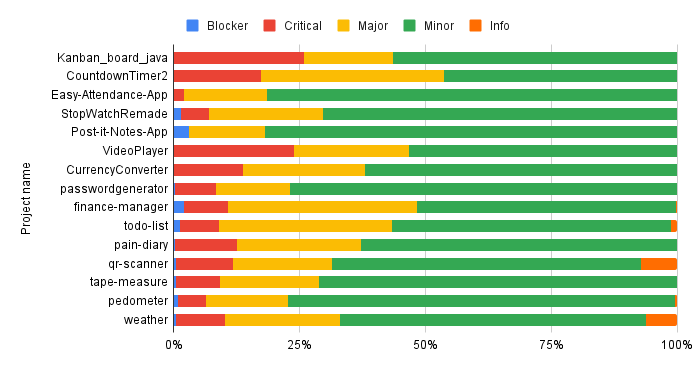
\includegraphics[scale = 0.58]{img/JAVASOLO.png}
    \caption{Severity Distribution in Java Projects}
    \label{fig:javasolo}
\end{figure}

\subsubsection{Kotlin Project Analysis}
Kotlin projects showed a slightly lower total LOC at 48,865 but had a significantly lower total of 647 code smells. This reflects a more efficient codebase overall. However, the proportion of Critical issues was higher at 18.9\%, as shown in Figure \ref*{fig:kotlinsolo} and Figure \ref*{fig:totalsolo}, indicating that while the codebases are generally efficient, there are critical areas requiring mitigation to avoid potential vulnerabilities. Minor issues were 50.2\%, major issues were 27\%, and info issues were 3.9\%, with no blocker issues recorded.


\begin{figure}[htbp]
    \centering
    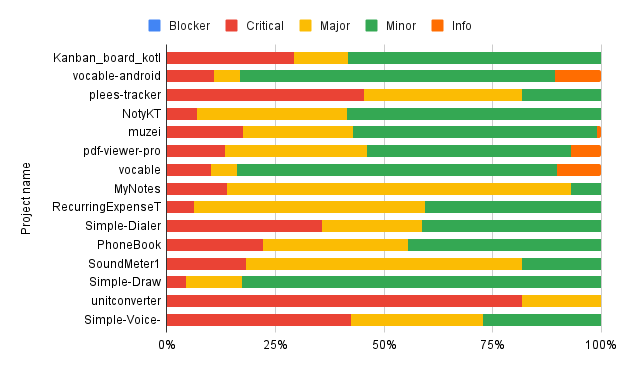
\includegraphics[scale = 0.58]{img/KOTLINSOLO.png}
    \caption{Severity Distribution in Kotlin Projects}
    \label{fig:kotlinsolo}
\end{figure}

\begin{figure}[htbp]
    \centering
    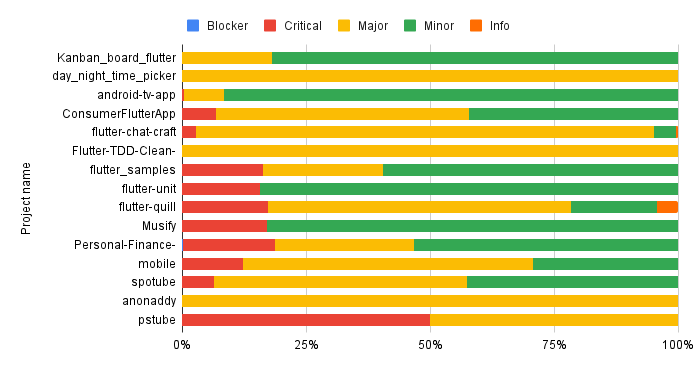
\includegraphics[scale = 0.58]{img/FLUTTERSOLO.png}
    \caption{Severity Distribution in Dart Projects}
    \label{fig:dartsolo}
\end{figure}
\subsubsection{Flutter Projects Analysis}
Flutter projects, using Dart for business logic and UI instead of XML as in Kotlin/Java, exhibited a significantly larger total LOC at 174,044 but managed a relatively modest total of 1,303 code smells. The distribution favors Minor code smells at 58.8\% and Major issues at 34.8\%, underscoring Flutter's ability to manage larger codebases effectively. Critical issues were notably lower at 6.1\%, and Info issues were minimal at 0.2\%, as illustrated in Figure \ref{fig:dartsolo} and Figure \ref*{fig:totalsolo}. This distribution highlights Flutter's capability to handle complex application development with fewer critical issues.
 

\begin{figure}[htbp]
    \centering
    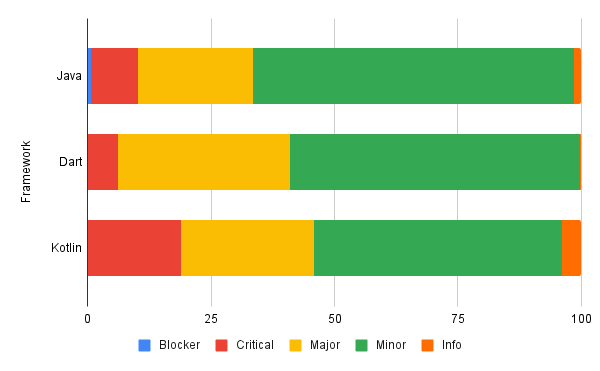
\includegraphics[scale = 0.58]{img/totalsolo.png}
    \caption{Severity Distribution of Code Smells Across Frameworks}
    \label{fig:totalsolo}
\end{figure}
\subsubsection{Comparative Graph and Discussion}
The comparative analysis, depicted in Figure \ref{fig:totalsolo}, combines the data from Java, Kotlin, and Flutter projects, clearly visualizing how each framework performs in managing code quality across different severity levels. This graph allows for a direct comparison and offers insights into the overall efficiency and security posture of applications developed under these frameworks.
\par
The analysis shows that while Java has the highest number of code smells, it also has a significant foundation that may contribute to higher Minor and Major issues. Kotlin, with its efficient but critical-prone codebase, offers a middle ground. In contrast, Flutter maintains a large codebase with a lower incidence of critical issues, proving its robustness in handling complex applications. This comprehensive view helps underline the strengths and weaknesses of each framework, guiding developers in choosing the most suitable technology based on the specific needs of their projects.
